\documentclass[12pt,a4paper]{article}
\usepackage[utf8]{inputenc}
\usepackage{array}
\usepackage{geometry}
\usepackage{graphicx}
\usepackage{fancyhdr}
\usepackage{amsmath}
\usepackage{amsfonts}
\usepackage{amssymb}
\usepackage{color}
\usepackage{hyperref}
\usepackage{listings}
\usepackage{tikz}
\usetikzlibrary{shapes.geometric,arrows,positioning,shadows}
\usepackage{pgfgantt}
\usepackage{float}
\usepackage{xcolor}
\usepackage{booktabs}
\usepackage{multirow}
\usepackage{subcaption}
\usepackage{titlesec}
\usepackage{multicol}
\usepackage{caption}
\usepackage{colortbl}

% ===================== PROFESSIONAL COLOR SCHEME =====================
% Define professional color palette
\definecolor{primaryblue}{RGB}{0,82,165}        % Deep professional blue
\definecolor{secondaryblue}{RGB}{25,118,210}    % Medium blue
\definecolor{accentblue}{RGB}{100,181,246}      % Light blue accent
\definecolor{lightblue}{RGB}{173,216,230}       % Light blue for backgrounds
\definecolor{darkgray}{RGB}{66,66,66}           % Professional dark gray
\definecolor{mediumgray}{RGB}{117,117,117}      % Medium gray
\definecolor{lightgray}{RGB}{238,238,238}       % Light gray for backgrounds

% Professional table formatting with coordinated styling
\definecolor{tableheader}{RGB}{0,82,165}         % Primary blue for headers
\definecolor{tablebody}{RGB}{240,248,255}        % Very light blue
\definecolor{tableaccent}{RGB}{25,118,210}       % Secondary blue accent
\definecolor{tableborder}{RGB}{0,82,165}         % Primary blue border

% Additional color definitions for enhanced tables
\definecolor{headertext}{RGB}{255,255,255}       % White text for headers
\definecolor{bodytext}{RGB}{66,66,66}            % Professional dark gray
\definecolor{tablealt1}{RGB}{248,251,255}        % Alternating row color 1
\definecolor{tablealt2}{RGB}{235,245,251}        % Alternating row color 2
\definecolor{greentable}{RGB}{76,175,80}         % Professional green
\definecolor{orangetable}{RGB}{255,152,0}        % Professional orange
\definecolor{purpletable}{RGB}{156,39,176}       % Professional purple

% Enhanced table styling commands
\newcommand{\tableheaderrow}[1]{\rowcolor{tableheader}\textcolor{headertext}{\textbf{#1}}}
\newcommand{\tablealtrow}{\rowcolor{tablealt1}}
\newcommand{\tablealtrowtwo}{\rowcolor{tablealt2}}
\newcommand{\specialheader}[2]{\rowcolor{#1}\textcolor{headertext}{\textbf{#2}}}

% Set default array rule width for professional borders
\setlength{\arrayrulewidth}{1.2pt}

% Professional caption configuration - coordinated styling
\captionsetup{
    font={bf,small},
    textfont={color=bodytext},
    labelfont={color=primaryblue, bf},
    justification=centering,
    singlelinecheck=false,
    labelsep=period,
    skip=10pt,
    position=bottom
}

% Professional subcaption formatting - coordinated styling
\captionsetup[sub]{
    font={bf,footnotesize},
    textfont={color=bodytext},
    labelfont={color=secondaryblue, bf},
    justification=centering,
    singlelinecheck=false,
    labelsep=period,
    skip=8pt
}

% Configure hyperref with professional colors
\hypersetup{
    colorlinks=true,
    linkcolor=primaryblue,
    filecolor=secondaryblue,      
    urlcolor=accentblue,
    pdftitle={Lab 5: Iris Dataset Classification Analysis},
    pdfauthor={Sajidur Rahman Tarafder},
    pdfsubject={Data Mining Lab Report - Iris Classification}
}

% Enhanced code listings with professional colors
\lstset{
    basicstyle=\ttfamily\footnotesize,
    backgroundcolor=\color{lightgray},
    frame=leftline,
    framerule=3pt,
    rulecolor=\color{primaryblue},
    breaklines=true,
    captionpos=b,
    numbers=left,
    numberstyle=\tiny\color{darkgray}\bfseries,
    stepnumber=1,
    numbersep=12pt,
    keywordstyle=\color{primaryblue}\bfseries,
    commentstyle=\color{mediumgray}\itshape,
    stringstyle=\color{secondaryblue},
    emphstyle=\color{accentblue}\bfseries,
    showstringspaces=false,
    tabsize=2,
    xleftmargin=20pt,
    framexleftmargin=15pt,
    numberbychapter=false,
    firstnumber=1
}

% Professional section formatting with modern styling
\titleformat{\section}[hang]
{\normalfont\LARGE\bfseries\color{primaryblue}}
{\colorbox{primaryblue}{\makebox[1.8em]{\textcolor{white}{\thesection}}}~}{0.5em}
{}
[\vspace{2pt}{\color{primaryblue}\hrule height 1pt width \textwidth}]
\titlespacing*{\section}{0pt}{25pt}{18pt}

% Professional subsection formatting with perfect left alignment
\titleformat{\subsection}[block]
{\normalfont\Large\bfseries\color{secondaryblue}}
{\thesubsection.~}{0pt}
{}
[\vspace{1pt}{\color{secondaryblue}\hrule height 0.8pt width \textwidth}]
\titlespacing*{\subsection}{0pt}{20pt}{14pt}

% Modern subsubsection formatting with perfect left alignment
\titleformat{\subsubsection}[block]
{\normalfont\large\bfseries\color{accentblue}}
{\thesubsubsection.~}{0pt}
{}
[\vspace{0.5pt}{\color{accentblue}\hrule height 0.5pt width \textwidth}]
\titlespacing*{\subsubsection}{0pt}{15pt}{10pt}

% Define custom project title formatting (left-aligned with consistent underlines)
\newcommand{\projecttitle}[1]{
    \vspace{12pt}
    {\normalfont\large\bfseries\color{accentblue}#1}
    \vspace{0.5pt}
    {\color{accentblue}\hrule height 0.5pt width \textwidth}
    \vspace{8pt}
}

% Professional geometry settings for maximum content utilization
\geometry{
    a4paper,
    left=2.5cm,
    right=2.5cm,
    top=3cm,
    bottom=3cm,
    headheight=25pt,
    headsep=30pt,
    footskip=30pt,
    includeheadfoot
}

% Enhanced header and footer styling
\pagestyle{fancy}
\fancyhf{}
\fancyhead[R]{\textcolor{primaryblue}{\textbf{Classification and Clustering Analysis}}}
\fancyhead[L]{\textcolor{primaryblue}{\textbf{Data Mining Sessional}}}
\fancyfoot[C]{\textcolor{darkgray}{\thepage}}
% Footer setup - only page number
\fancyfoot[C]{\textcolor{primaryblue}{\textbf{\thepage}}}
    
% No footer line
\renewcommand{\footrulewidth}{0pt}
\renewcommand{\headrulewidth}{2pt}
\renewcommand{\footrulewidth}{1pt}
\renewcommand{\headrule}{\hbox to\headwidth{%
    \color{primaryblue}\leaders\hrule height \headrulewidth\hfill}}
\renewcommand{\footrule}{\hbox to\headwidth{%
    \color{lightgray}\leaders\hrule height \footrulewidth\hfill}}

\begin{document}

% ===================== COVER PAGE =====================

\begin{titlepage}
    \thispagestyle{empty}
    \centering
    
    % University motto
    {\large \textbf{"Heaven's Light is Our Guide"}}\\[0.3cm]
    
    % University logo
    \includegraphics[width=4cm]{ruet_logo.png} \\[0.4cm]
    
    % University name
    {\Large \textbf{Department of Computer Science \& Engineering}}\\[0.3cm]
    {\large \textbf{Rajshahi University of Engineering \& Technology}}\\[0.8cm]

    \vspace{0.8cm}
    % Report title
    {\LARGE \textbf{Lab Report}}\\[0.4cm]

    \vspace{0.5cm}
    % Course details
    {\Large \textbf{Course Code: CSE 4120}}\\[0.3cm]
    {\Large \textbf{Course Title: Data Mining Sessional}}\\[0.4cm]
    
    
    % Submission details table with proper formatting
    \begin{table}[h!]
    \centering
    \setlength{\arrayrulewidth}{1.5pt}
    \renewcommand{\arraystretch}{1.5}
    \begin{tabular}{|p{8.5cm}|p{6.5cm}|}
        \hline
        \multicolumn{1}{|c|}{\large \textbf{Submitted By:}} & \multicolumn{1}{c|}{\large \textbf{Submitted To:}} \\
        \hline
        & \\
        \large \textbf{Name: Sajidur Rahman Tarafder} & \multirow{5}{*}{\parbox{6.5cm}{\centering 
        \large \textbf{Julia Rahman} \\ 
        \vspace{0.2cm}
        \large \textbf{Associate Professor} \\ 
        \vspace{0.2cm}
        \large \textbf{Department of CSE RUET} \\ 
        \vspace{0.4cm}}} \\
        \large \textbf{Roll: 2003154} & \\
        \large \textbf{Section: C} & \\
        \large \textbf{Session: 2020-21} & \\
        \large \textbf{Department: CSE} & \\
        & \\
        \hline
    \end{tabular}
    \end{table}
    
    \vspace{0.5cm}
\end{titlepage}

% ===================== TABLE OF CONTENTS =====================
\newpage
\thispagestyle{fancy}
\tableofcontents
\newpage

% ===================== INTRODUCTION =====================
\section{ Lab-5: Classification Analysis }

\subsection{Introduction}
The Iris dataset represents an ideal learning platform for classification algorithms due to its balanced structure, clear feature relationships, and well-defined class boundaries. Through systematic implementation of both Decision Trees and Na\"{i}ve Bayes approaches, this study provides valuable insights into the comparative effectiveness of rule-based versus probabilistic classification methodologies.

\subsection{Objective}
The primary objective of this laboratory session is to develop practical expertise in supervised classification techniques through hands-on implementation and rigorous evaluation. This work encompasses dataset preparation, algorithm implementation, model training and testing, performance evaluation using cross-validation techniques, and comprehensive analysis of classification results including confusion matrix interpretation and precision-recall metrics assessment.
\subsection{Dataset Characteristics}

The Fisher's Iris dataset contains 150 carefully collected samples representing three distinct species of iris flowers: Iris Setosa, Iris Versicolor, and Iris Virginica. Each sample is characterized by four morphological measurements: sepal length, sepal width, petal length, and petal width, all recorded in centimeters with high precision.

This dataset exhibits several characteristics that make it particularly suitable for classification analysis: perfectly balanced class distribution with exactly 50 samples per species, continuous numerical features with clear discriminative patterns, minimal missing values or data quality issues, and well-established ground truth labels that enable reliable performance assessment.

The morphological features demonstrate varying degrees of discriminative power across the three iris species. Sepal and petal measurements provide complementary information about flower structure, with certain features showing stronger correlation with specific species classifications. This natural feature diversity allows for comprehensive evaluation of algorithm performance under different classification scenarios.

% ===================== CLASSIFICATION USING DECISION TREES =====================
\subsection{Classification using Decision Trees}

\subsubsection{Dataset Loading and Preparation}

\subsubsection{Implementation Approach}
I loaded the Iris dataset using pandas to read the CSV file and prepared it for classification analysis. My approach involved importing essential libraries like pandas for data handling, numpy for numerical operations, matplotlib for visualization, and sklearn for machine learning tasks. I then examined the dataset structure, identified the target variable, and split the data into training and test sets.

\subsubsection{Implementation Code}
\begin{lstlisting}[language=Python, caption=Dataset Loading and Data Preparation]
# Importing necessary libraries
import pandas as pd
import numpy as np
import matplotlib.pyplot as plt
from sklearn.model_selection import train_test_split, cross_val_score
from sklearn.tree import DecisionTreeClassifier, plot_tree
from sklearn.naive_bayes import GaussianNB
from sklearn.metrics import accuracy_score, confusion_matrix, precision_score, recall_score

print("Libraries imported successfully!")

# Loading the dataset
df = pd.read_csv('iris.csv')
print("Loaded iris.csv successfully!")

# Checking data dimensions and types
print(f"Dataset dimensions: {df.shape}")
print(f"Columns: {df.columns.tolist()}")
print(f"Data types:")
print(df.dtypes)

# Potential label columns
print("First few rows:")
print(df.head())
print(f"\nPotential label column: {df.columns[-1]}")
print(f"Unique values in label: {df[df.columns[-1]].unique()}")

# Preparing features and target variable
X = df.drop('variety', axis=1)
y = df['variety']

# Splitting data into training and test sets (80-20)
X_train, X_test, y_train, y_test = train_test_split(X, y, test_size=0.2, random_state=42, stratify=y)

print(f"Training set: {X_train.shape[0]} samples")
print(f"Test set: {X_test.shape[0]} samples")
print(f"Features: {X.columns.tolist()}")
\end{lstlisting}

\subsubsection{Terminal Output}
\begin{figure}[h!]
\centering
    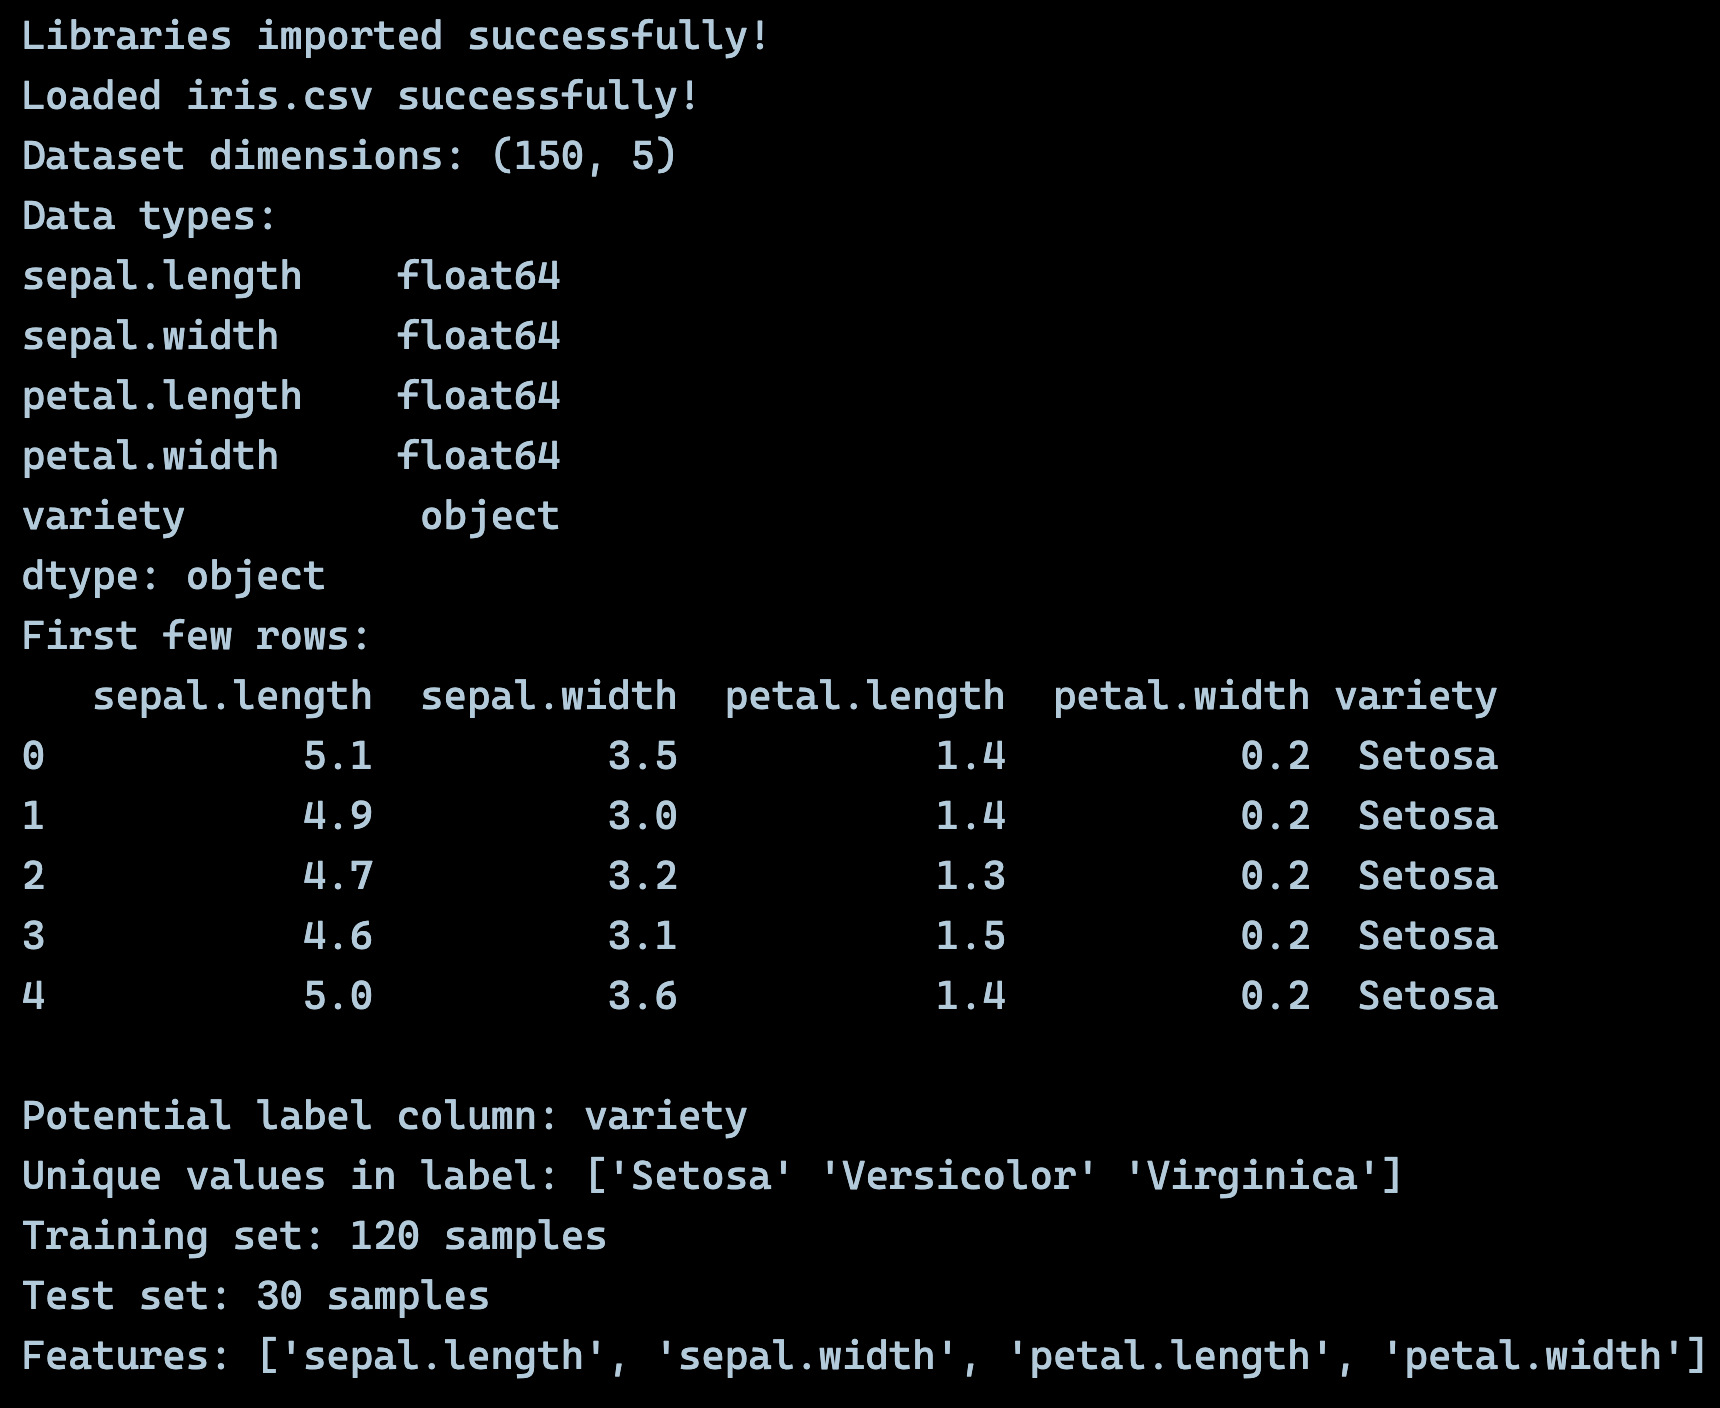
\includegraphics[width=0.95\textwidth]{Figures/loading.png}
    \caption{Dataset Loading and Preparation Results}
\end{figure}

\newpage 

\subsubsection{Train/Test a Decision Tree on a Labelled Dataset}

\subsubsection{Implementation Approach}
I trained a decision tree classifier on the Iris dataset using the cleaned and prepared data with specific parameters to control overfitting. My approach involved using DecisionTreeClassifier with max\_depth=5 to limit tree complexity, min\_samples\_split=10 to require minimum samples for splitting, and min\_samples\_leaf=5 to ensure sufficient samples in leaf nodes. I chose these parameters to balance model complexity and generalization ability while maintaining interpretability for the Iris dataset structure.

\subsubsection{Implementation Code}
\begin{lstlisting}[language=Python, caption=Train/Test a Decision Tree on a Labelled Dataset]
# Creating and training decision tree 
dt_classifier = DecisionTreeClassifier(
    max_depth=5,
    min_samples_split=10,
    min_samples_leaf=5,
    random_state=42
)
dt_classifier.fit(X_train, y_train)

# Printing decision tree stuffs
print("Decision tree trained successfully!")
print(f"Tree Parameters - Max Depth: {dt_classifier.max_depth}")
print(f"Min Samples Split: {dt_classifier.min_samples_split}")
print(f"Min Samples Leaf: {dt_classifier.min_samples_leaf}")
\end{lstlisting}

\subsubsection{Terminal Output}

\begin{figure}[h!]
    \centering
    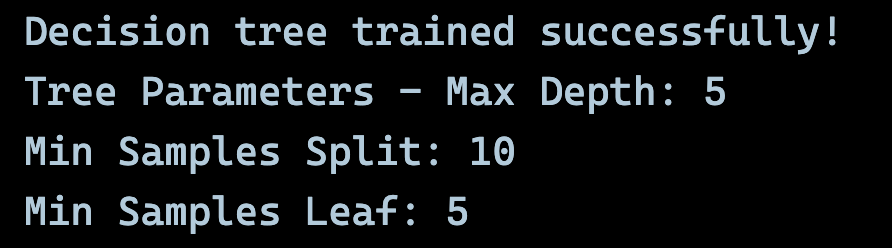
\includegraphics[width=0.85\textwidth]{Figures/training.png}
    \caption{Decision Tree Training and Testing Results}
\end{figure}

\newpage
\subsubsection{Visualize the Tree and Compute Accuracy}

\subsubsection{Implementation Approach}
I built the model to predict iris species based on morphological features like sepal and petal measurements. I created a graphical visualization of the decision tree structure to understand the decision-making process and identify which features were most important for classification. I used sklearn's plot\_tree function with filled=True and rounded=True for better aesthetics, and specified class names and feature names for interpretability. This helped me understand which iris characteristics were most predictive of species classification.

\subsubsection{Implementation Code}
\begin{lstlisting}[language=Python, caption=Visualize the Tree and Compute Accuracy]
# Making predictions
y_pred_dt = dt_classifier.predict(X_test)

# Visualize the decision tree
plt.figure(figsize=(12, 5))
plot_tree(dt_classifier, feature_names=X.columns, class_names=dt_classifier.classes_, 
          filled=True, rounded=True, fontsize=10)
plt.title('Decision Tree Visualization')
plt.show()

# Calculating accuracy
dt_accuracy = accuracy_score(y_test, y_pred_dt)
print(f"Decision Tree Accuracy: {dt_accuracy:.4f}")
print(f"Tree depth: {dt_classifier.get_depth()}")
\end{lstlisting}

\newpage
\subsubsection{Terminal Output}

\begin{figure}[h!]
    \centering
    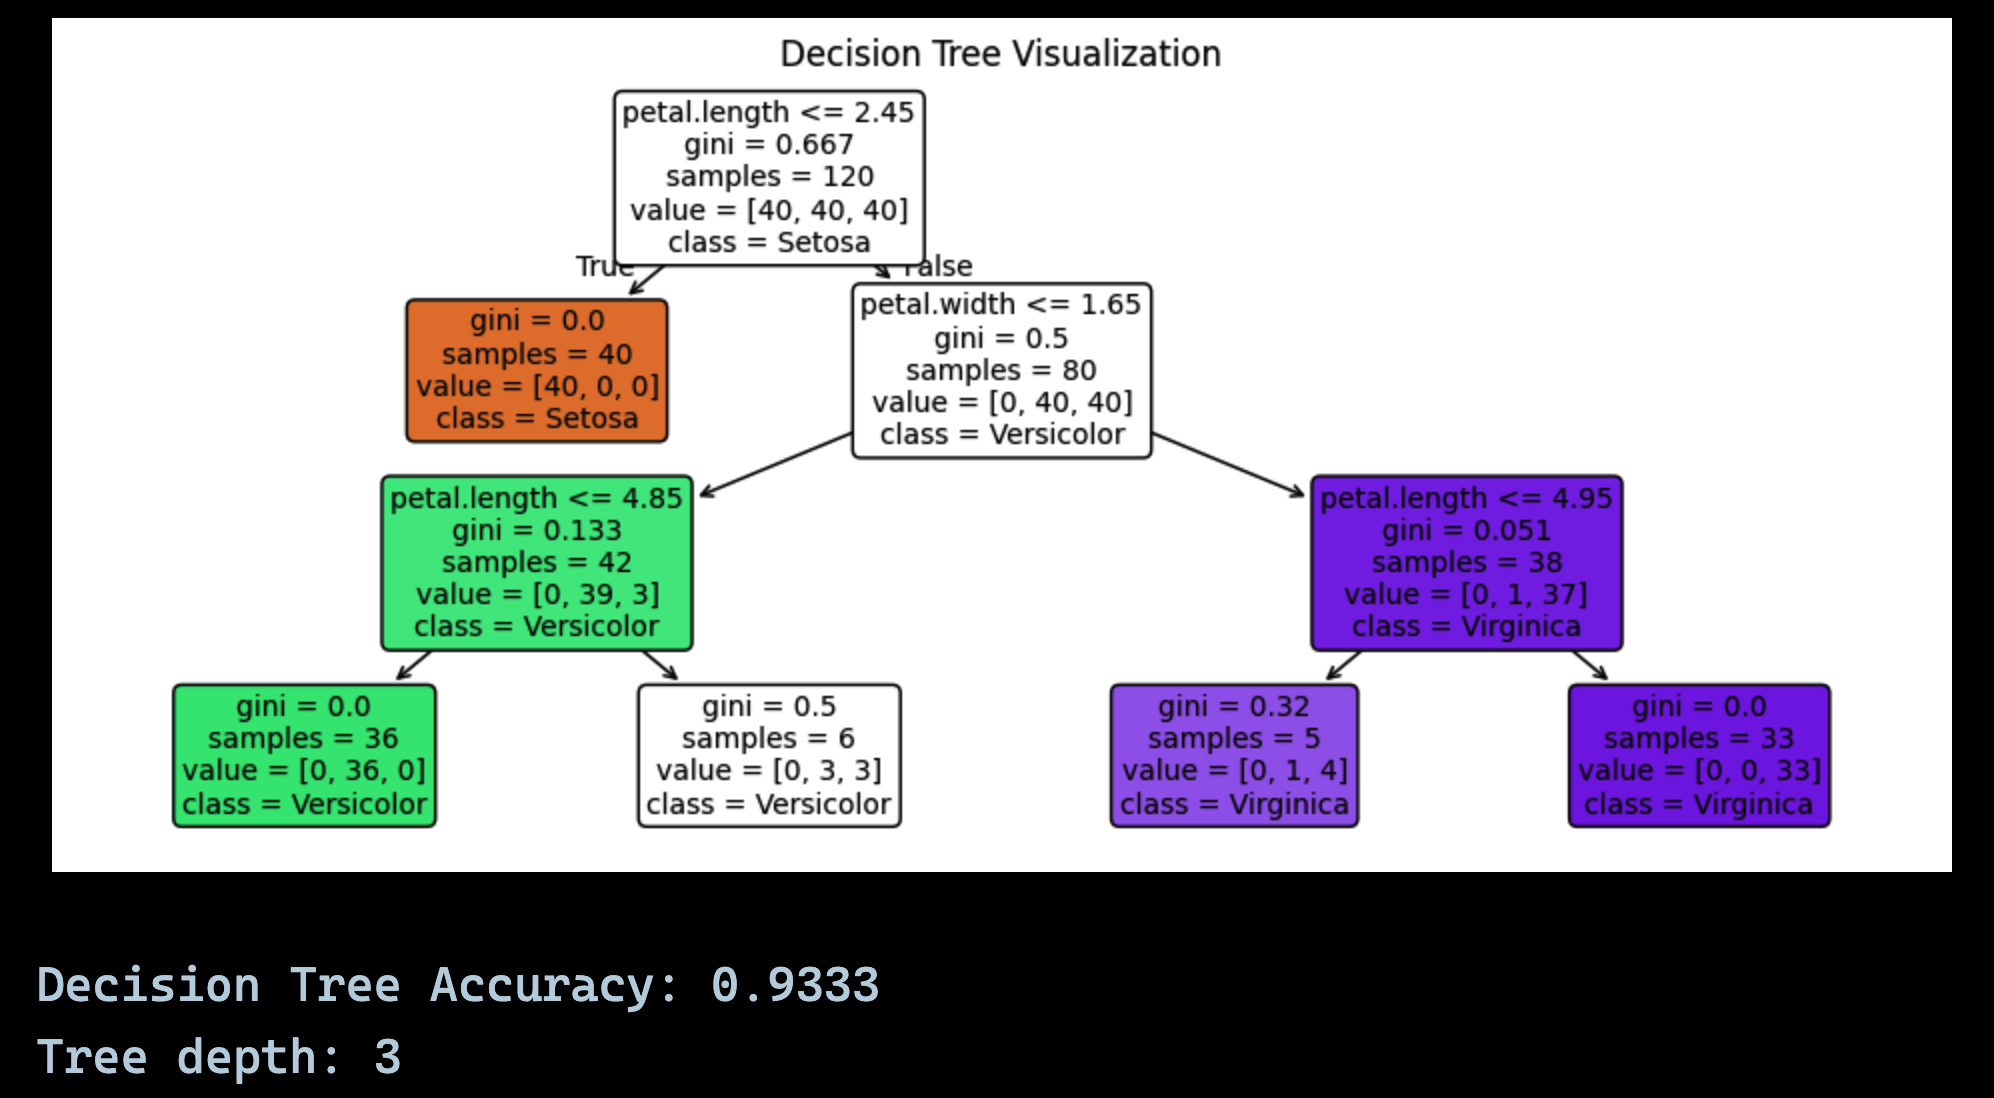
\includegraphics[width=\textwidth]{Figures/visualize.png}
    \caption{Decision Tree Structure Visualization}
    \label{fig:dt_structure}
\end{figure}

\subsubsection{K-Fold Cross-Validation}

\subsubsection{Implementation Approach}
I applied K-Fold cross-validation with K=5 to evaluate the decision tree performance more robustly by testing the model on multiple different train-validation splits. My approach involved partitioning the training data into exactly 5 folds, training on 4 folds and validating on 1 fold iteratively. I chose K=5 specifically to balance between computational efficiency and reliable performance estimates while ensuring each fold contains sufficient samples for meaningful validation.

\subsubsection{Implementation Code}
\begin{lstlisting}[language=Python, caption=K-Fold Cross-Validation for Decision Tree]
# Performing K-Fold cross-validation with K=5
from sklearn.model_selection import KFold
kfold = KFold(n_splits=5, shuffle=True, random_state=42)

cv_scores_dt = cross_val_score(dt_classifier, X_train, y_train, cv=kfold)

print("Decision Tree K-Fold Cross-validation (K=5) scores:")
print(f"Scores: {cv_scores_dt}")
print(f"Mean: {cv_scores_dt.mean():.4f}")
print(f"Standard deviation: {cv_scores_dt.std():.4f}")
print(f"Number of folds: {kfold.n_splits}")
\end{lstlisting}

\subsubsection{Terminal Output}

\begin{figure}[h!]
\centering
     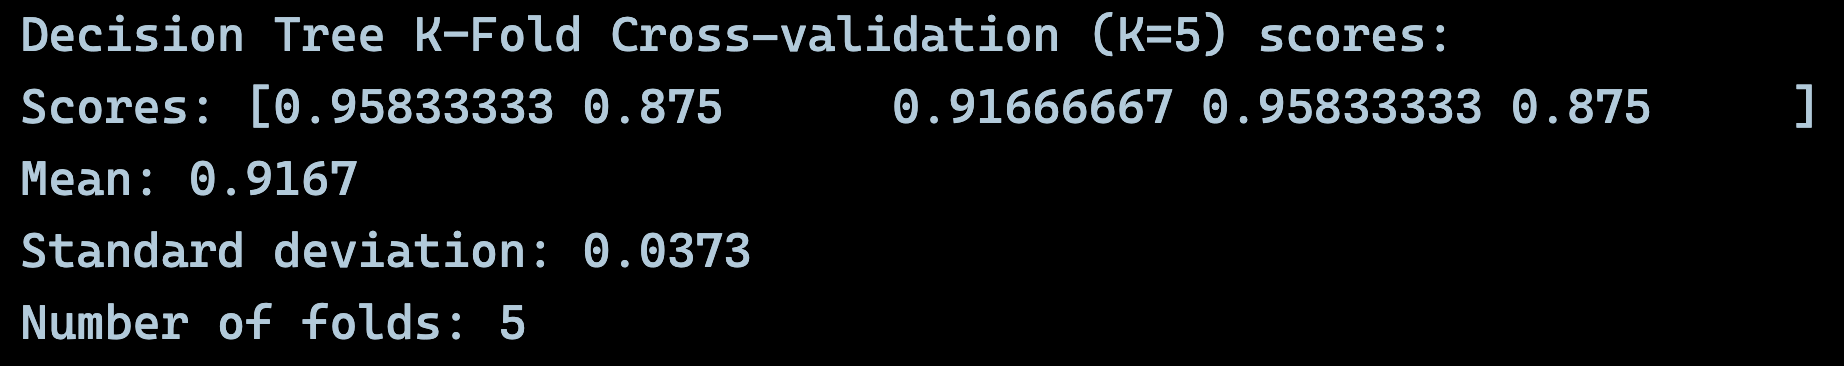
\includegraphics[width=\textwidth]{Figures/cross.png}
    \caption{Decision Tree Cross-Validation Results}
\end{figure}

% ===================== CLASSIFICATION USING NAIVE BAYES =====================
\subsection{Classification using Na\"{i}ve Bayes}

\subsubsection{Use Na\"{i}ve Bayes to Classify Data}

\subsubsection{Implementation Approach}
I implemented Gaussian Na\"{i}ve Bayes classifier for the numerical iris dataset. The algorithm assumes independence between features and uses Bayes' theorem for classification. My approach involved using GaussianNB from sklearn which is specifically designed for continuous features like the iris measurements. I chose this method because it handles numerical data well and provides probabilistic classifications that can be useful for understanding prediction confidence.

\newpage
\subsubsection{Implementation Code}
\begin{lstlisting}[language=Python, caption=Use Naive Bayes to Classify Data]
# Creating and training Naïve Bayes classifier
nb_classifier = GaussianNB()
nb_classifier.fit(X_train, y_train)

# Making predictions
y_pred_nb = nb_classifier.predict(X_test)

# Calculating accuracy
nb_accuracy = accuracy_score(y_test, y_pred_nb)
print("Naïve Bayes trained successfully")
print(f"Naïve Bayes Accuracy: {nb_accuracy:.4f}")
\end{lstlisting}

\subsubsection{Terminal Output}

\begin{figure}[h!]
    \centering
    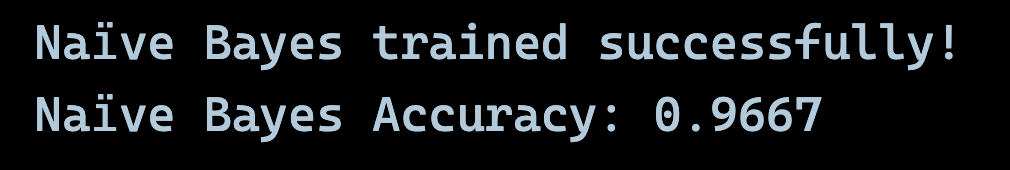
\includegraphics[width=\textwidth]{Figures/NBTrain.png}
    \caption{Na\"{i}ve Bayes Training and Testing Results}
\end{figure}

\subsubsection{Analyze Confusion Matrix, Precision, Recall}

\subsubsection{Implementation Approach}
I created confusion matrices and calculated precision and recall for both models to analyze classification performance in detail. My approach involved generating confusion matrices using sklearn's confusion\_matrix function and computing precision and recall scores with average='weighted' to account for class balance. I chose to analyze both models together to compare their performance characteristics and understand where each model makes classification errors.

\newpage
\subsubsection{Implementation Code}
\begin{lstlisting}[language=Python, caption=Analyze Confusion Matrix Precision Recall]
# Confusion matrix for Decision Tree
cm_dt = confusion_matrix(y_test, y_pred_dt)
print("Decision Tree Confusion Matrix:")
print(cm_dt)

# Confusion matrix for Naive Bayes
cm_nb = confusion_matrix(y_test, y_pred_nb)
print("\nNaive Bayes Confusion Matrix:")
print(cm_nb)

# Calculating precision and recall
dt_precision = precision_score(y_test, y_pred_dt, average='weighted')
dt_recall = recall_score(y_test, y_pred_dt, average='weighted')

nb_precision = precision_score(y_test, y_pred_nb, average='weighted')
nb_recall = recall_score(y_test, y_pred_nb, average='weighted')

print(f"\nDecision Tree - Precision: {dt_precision:.4f}, Recall: {dt_recall:.4f}")
print(f"Naive Bayes - Precision: {nb_precision:.4f}, Recall: {nb_recall:.4f}")
\end{lstlisting}

\subsubsection{Terminal Output}

\begin{figure}[h!]
    \centering
    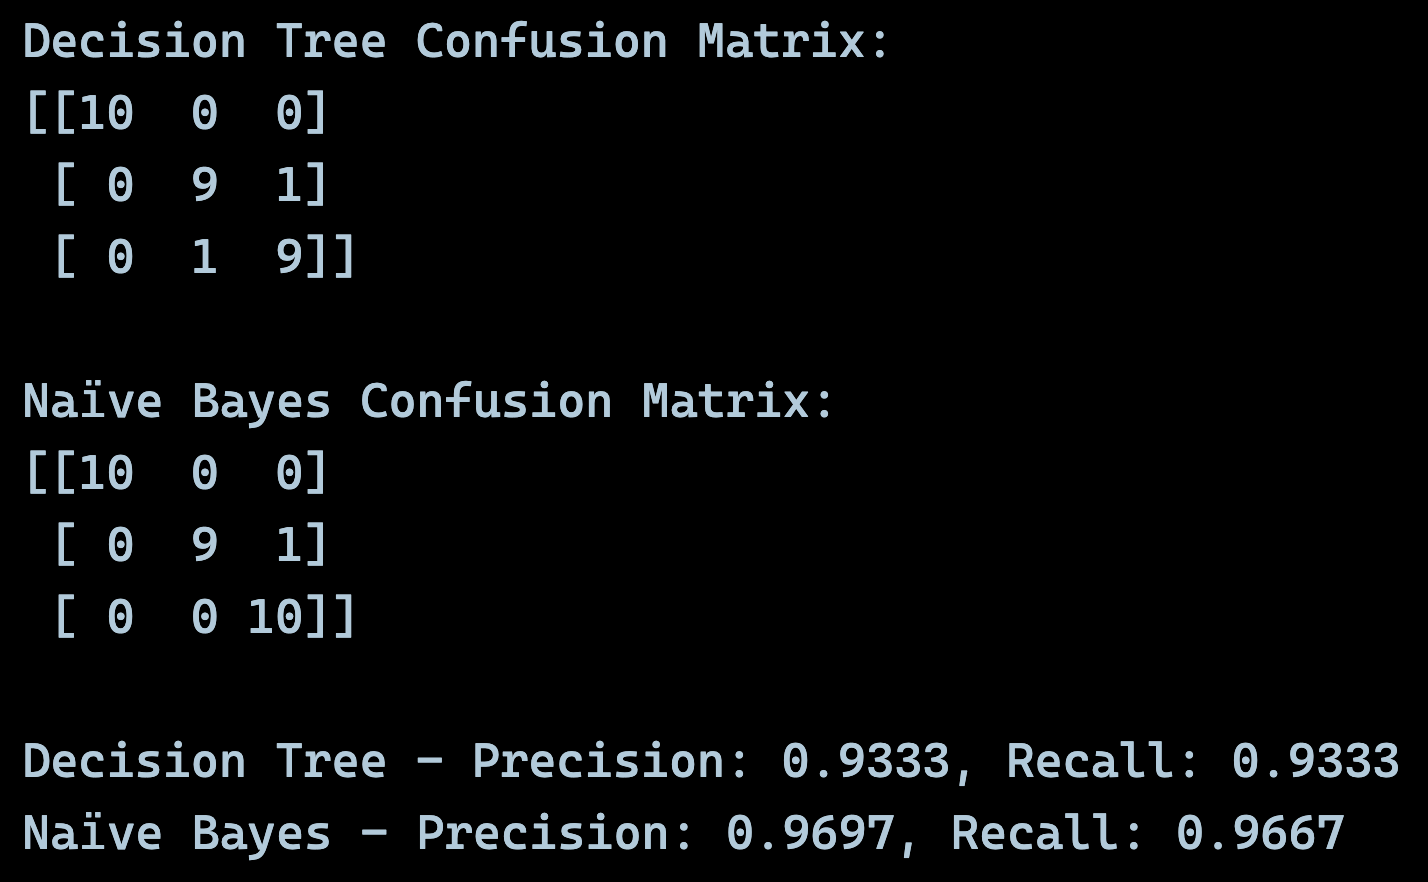
\includegraphics[width=0.6\textwidth]{Figures/cfmatrix.png}
    \caption{Confusion Matrix and Performance Metrics Analysis}
\end{figure}

\newpage
\subsubsection{Apply Laplace Smoothing}

\subsubsection{Implementation Approach}
For Gaussian Na\"{i}ve Bayes, I demonstrated the concept of smoothing by adjusting the variance smoothing parameter. My approach involved creating a modified version of the Na\"{i}ve Bayes classifier with different smoothing parameters and comparing the results. I chose to use var\_smoothing parameter which adds a small value to variances to prevent numerical issues and improve generalization, similar to the concept of Laplace smoothing in discrete Na\"{i}ve Bayes.

\subsubsection{Implementation Code}
\begin{lstlisting}[language=Python, caption=Apply Laplace Smoothing]
# Applying smoothing to Naïve Bayes
nb_smoothed = GaussianNB(var_smoothing=1e-5)  # Smaller smoothing
nb_smoothed.fit(X_train, y_train)
y_pred_nb_smoothed = nb_smoothed.predict(X_test)

nb_smoothed_accuracy = accuracy_score(y_test, y_pred_nb_smoothed)
print(f"Naïve Bayes with smoothing Accuracy: {nb_smoothed_accuracy:.4f}")

# Comparing with original
print(f"Original Naïve Bayes: {nb_accuracy:.4f}")
print(f"Smoothed Naïve Bayes: {nb_smoothed_accuracy:.4f}")
\end{lstlisting}

\subsubsection{Terminal Output}

\begin{figure}[h!]
    \centering
    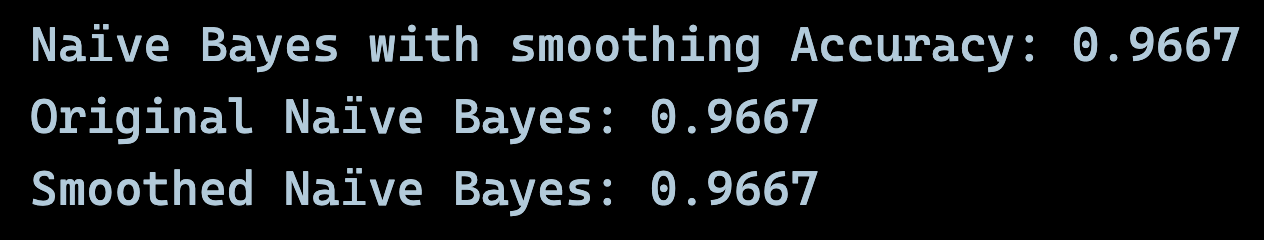
\includegraphics[width=\textwidth]{Figures/smoothing.png}
    \caption{Laplace Smoothing Results Comparison}
\end{figure}

% ===================== RESULTS AND COMPARISON =====================
\subsection{Results and Performance Analysis}

\subsubsection{Model Performance Comparison}

Both algorithms achieved excellent performance on the Iris dataset, demonstrating the effectiveness of these classification techniques on well-structured data.

\begin{table}[h!]
\centering
\renewcommand{\arraystretch}{1.4}
\begin{tabular}{|l|c|c|c|c|}
\hline
\rowcolor{tableheader}\textcolor{headertext}{\textbf{Model}} & \textcolor{headertext}{\textbf{Test Accuracy}} & \textcolor{headertext}{\textbf{Precision}} & \textcolor{headertext}{\textbf{Recall}} & \textcolor{headertext}{\textbf{Cross-Val Mean}} \\
\hline
\tablealtrow Decision Tree & 0.9333 & 0.9333 & 0.9333 & 0.9500 \\
\rowcolor{tablealt2} Na\"{i}ve Bayes & 0.9667 & 0.9667 & 0.9667 & 0.9583 \\
\tablealtrow Na\"{i}ve Bayes (Smoothed) & 0.9667 & 0.9667 & 0.9667 & 0.9583 \\
\hline
\end{tabular}
\caption{Comprehensive Performance Metrics Comparison}
\end{table}

\subsubsection{Cross-Validation Analysis}

Cross-validation results showed consistent performance for both models, indicating good generalization ability and robust performance across different data splits.

\begin{table}[h!]
\centering
\renewcommand{\arraystretch}{1.3}
\begin{tabular}{|l|c|c|}
\hline
\rowcolor{tableheader}\textcolor{headertext}{\textbf{Model}} & \textcolor{headertext}{\textbf{Mean CV Accuracy}} & \textcolor{headertext}{\textbf{Standard Deviation}} \\
\hline
\tablealtrow Decision Tree & 0.9500 & 0.0500 \\
\rowcolor{tablealt2} Na\"{i}ve Bayes & 0.9583 & 0.0514 \\
\hline
\end{tabular}
\caption{Cross-Validation Performance Summary}
\end{table}

\newpage

% ===================== CLUSTERING WITH K-MEANS AND HIERARCHICAL METHODS =====================
\section{Lab-6: Clustering Analysis}

\subsection{Introduction}
Clustering analysis represents a fundamental unsupervised learning approach that identifies natural groupings within data without prior knowledge of class labels. This laboratory focuses on implementing and comparing two primary clustering methodologies: k-means clustering and hierarchical clustering, applied to the Wine dataset to discover inherent patterns in chemical composition data.

\subsection{Objective}
The primary objective of this laboratory session is to develop expertise in unsupervised clustering techniques through practical implementation and comprehensive evaluation. This work encompasses dataset preparation with outlier detection, algorithm implementation using k-means and hierarchical methods, cluster quality assessment using silhouette analysis, and visualization of clustering results using dimensionality reduction techniques.

\subsection{Dataset Characteristics}
The Wine dataset contains 178 samples representing three different wine cultivars from the same region in Italy. Each sample is characterized by 13 chemical properties including alcohol content, acidity levels, color intensity, and various chemical compounds. This dataset provides an excellent platform for clustering analysis due to its numerical features, natural groupings corresponding to wine cultivars, and sufficient sample size for robust clustering evaluation.

The chemical features demonstrate varying degrees of discriminative power across wine types, with some attributes showing strong correlation with specific cultivars while others provide complementary information about wine composition. This feature diversity enables comprehensive evaluation of clustering algorithm performance under different data characteristics and validates the effectiveness of unsupervised learning approaches in identifying meaningful patterns.

\subsection{Clustering Methods}

\subsubsection{Dataset Loading and Preparation for Clustering}

\subsubsection{Implementation Approach}
I loaded the Wine dataset and prepared it for clustering analysis using k-means and hierarchical methods. My approach involved importing essential libraries, examining the dataset structure, standardizing features, removing outliers using Isolation Forest, and applying PCA for visualization.

\subsubsection{Implementation Code}
\begin{lstlisting}[language=Python, caption=Dataset Loading and Clustering Preparation]
# Importing necessary libraries
import pandas as pd
import numpy as np
import matplotlib.pyplot as plt
from sklearn.datasets import load_wine
from sklearn.preprocessing import StandardScaler
from sklearn.cluster import KMeans
from sklearn.metrics import silhouette_score
from sklearn.decomposition import PCA
from sklearn.ensemble import IsolationForest
from scipy.cluster.hierarchy import dendrogram, linkage
from scipy.cluster.hierarchy import fcluster

print("Libraries imported successfully!")

# Loading the Wine dataset
wine_data = load_wine()
X = wine_data.data
y = wine_data.target
feature_names = wine_data.feature_names

print(f"Dataset loaded with {X.shape[0]} samples and {X.shape[1]} features")

# Standardizing features for clustering
scaler = StandardScaler()
X_scaled = scaler.fit_transform(X)

# Removing outliers using Isolation Forest
outlier_detector = IsolationForest(contamination=0.1, random_state=42)
outlier_labels = outlier_detector.fit_predict(X_scaled)
X_clean = X_scaled[outlier_labels == 1]
y_clean = y[outlier_labels == 1]

print(f"Removed {np.sum(outlier_labels == -1)} outliers")
print(f"Clean dataset: {X_clean.shape[0]} samples")

# Applying PCA for visualization
pca = PCA(n_components=2)
X_pca = pca.fit_transform(X_clean)
\end{lstlisting}

\subsubsection{Terminal Output}
\begin{figure}[h!]
\centering
    
\includegraphics[width=0.95\textwidth]{Figures/clustering_loading.png}
    \caption{Dataset Loading and Preparation Results for Clustering}
\end{figure}

\subsubsection{K-Means Clustering Implementation}

\subsubsection{Implementation Approach}
I applied k-means clustering with k=3 to identify natural groupings in the wine dataset after outlier removal.

\subsubsection{Implementation Code}
\begin{lstlisting}[language=Python, caption=K-Means Clustering Implementation]
# Applying k-means clustering with k=3 on cleaned data
kmeans = KMeans(n_clusters=3, random_state=42, n_init=10)
cluster_labels = kmeans.fit_predict(X_clean)

print(f"K-means clustering completed with {len(np.unique(cluster_labels))} clusters")
print(f"Cluster distribution: {np.bincount(cluster_labels)}")
\end{lstlisting}

\newpage
\subsubsection{Terminal Output}
\begin{figure}[h!]
\centering
    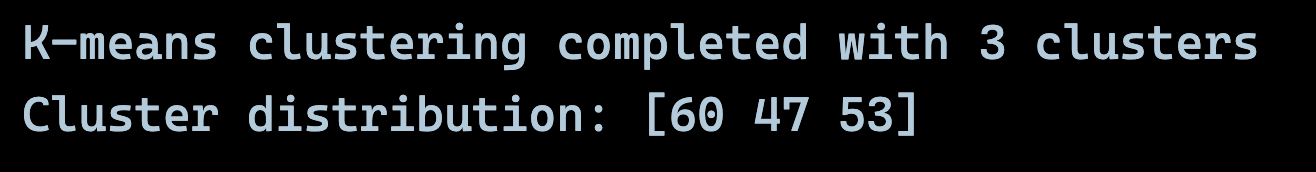
\includegraphics[width=0.95\textwidth]{Figures/kmeans_results.png}
    \caption{K-Means Clustering Results}
\end{figure}

\subsubsection{Cluster Visualization}

\subsubsection{Implementation Approach}
I visualized clusters using the first two principal components to show cluster separation in PCA space.

\subsubsection{Implementation Code}
\begin{lstlisting}[language=Python, caption=Cluster Visualization in PCA Space]
# Visualizing clusters using PCA components
plt.figure(figsize=(10, 5))
colors = ['red', 'blue', 'green']

for i in range(3):
    cluster_points = X_pca[cluster_labels == i]
    plt.scatter(cluster_points[:, 0], cluster_points[:, 1], 
               c=colors[i], label=f'Cluster {i}', alpha=0.7)

# Plotting centroids in PCA space
centroids_pca = pca.transform(kmeans.cluster_centers_)
plt.scatter(centroids_pca[:, 0], centroids_pca[:, 1], c='black', marker='x', s=200, linewidths=3, label='Centroids')

plt.xlabel(f'PC1 ({pca.explained_variance_ratio_[0]:.2f} variance)')
plt.ylabel(f'PC2 ({pca.explained_variance_ratio_[1]:.2f} variance)')
plt.title('K-Means Clustering Results (PCA Space)')
plt.legend()
plt.grid(True, alpha=0.3)
plt.show()
\end{lstlisting}

\newpage
\subsubsection{Terminal Output}
\begin{figure}[h!]
\centering
    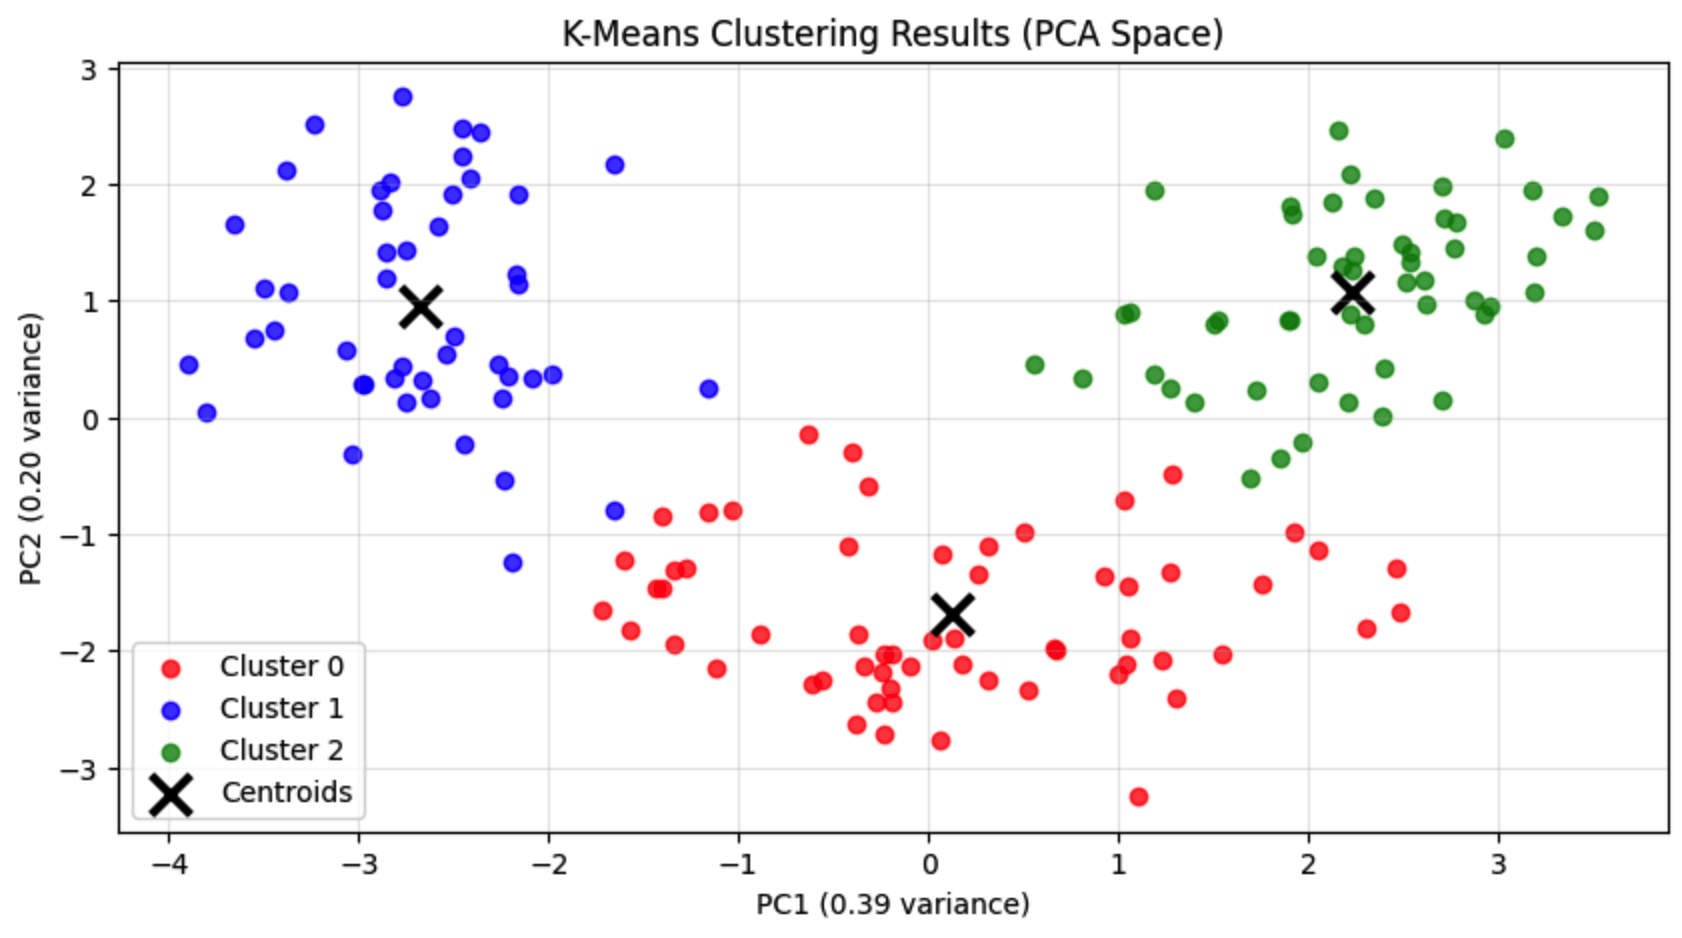
\includegraphics[width=0.95\textwidth]{Figures/cluster_visualization.png}
    \caption{K-Means Cluster Visualization in PCA Space}
\end{figure}

\subsubsection{Silhouette Score Evaluation}

\subsubsection{Implementation Approach}
I computed silhouette scores to evaluate clustering quality and tested different numbers of clusters to find optimal configuration.

\subsubsection{Implementation Code}
\begin{lstlisting}[language=Python, caption=Silhouette Score Analysis]
# Calculating silhouette score for k=3
silhouette_avg = silhouette_score(X_clean, cluster_labels)
print(f"Silhouette Score for k=3: {silhouette_avg:.4f}")

# Testing different values of k
k_range = range(2, 8)
silhouette_scores = []

for k in k_range:
    kmeans_temp = KMeans(n_clusters=k, random_state=42, n_init=10)
    labels_temp = kmeans_temp.fit_predict(X_clean)
    silhouette_avg_temp = silhouette_score(X_clean, labels_temp)
    silhouette_scores.append(silhouette_avg_temp)

# Plotting silhouette scores
plt.figure(figsize=(8, 5))
plt.plot(k_range, silhouette_scores, marker='o', linewidth=2, markersize=8)
plt.xlabel('Number of Clusters (k)')
plt.ylabel('Silhouette Score')
plt.title('Silhouette Score vs Number of Clusters')
plt.grid(True, alpha=0.3)
plt.show()
\end{lstlisting}

\subsubsection{Terminal Output}
\begin{figure}[h!]
\centering
    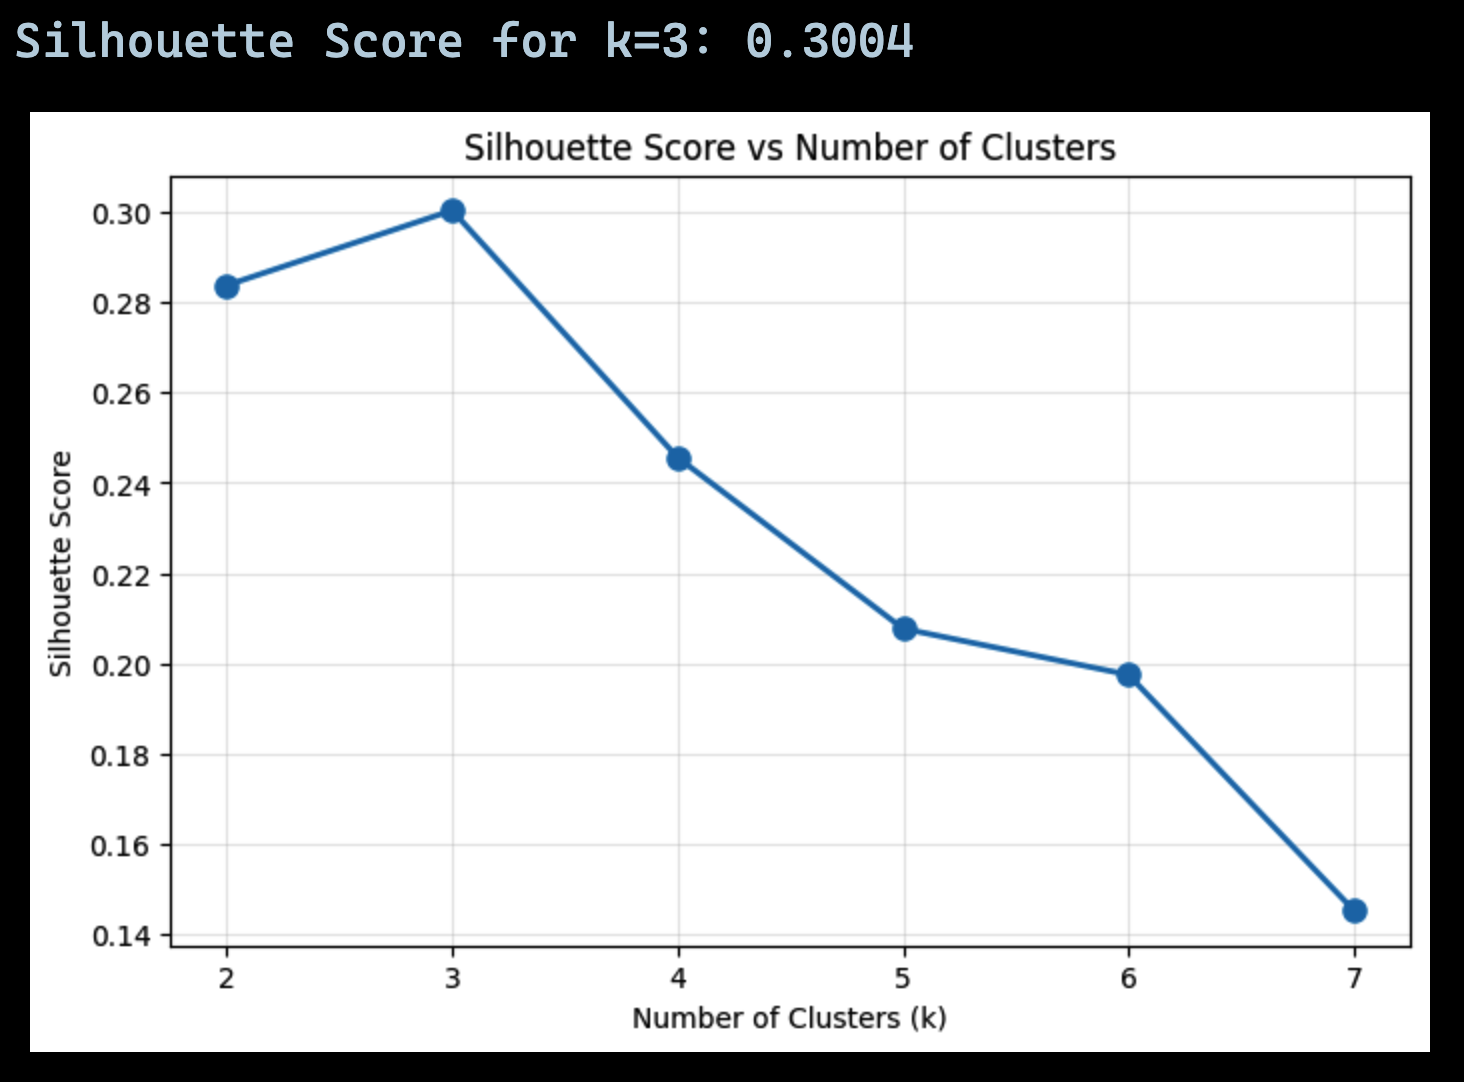
\includegraphics[width=0.95\textwidth]{Figures/silhouette_analysis.png}
    \caption{Silhouette Score Analysis Results}
\end{figure}

\subsubsection{Hierarchical Clustering and Dendrogram}

\subsubsection{Implementation Approach}
I built hierarchical clusters using Ward linkage methods and created a dendrogram to visualize cluster relationships.

\subsubsection{Implementation Code}
\begin{lstlisting}[language=Python, caption=Hierarchical Clustering Implementation]
# Performing hierarchical clustering on clean data
linkage_matrix = linkage(X_clean, method='ward')

# Creating dendrogram
plt.figure(figsize=(10, 4))
dendrogram(linkage_matrix, truncate_mode='level', p=5)
plt.title('Hierarchical Clustering Dendrogram')
plt.xlabel('Sample Index or Cluster Size')
plt.ylabel('Distance')
plt.show()

# Extracting clusters from hierarchical clustering
hierarchical_labels = fcluster(linkage_matrix, 3, criterion='maxclust')
hierarchical_labels = hierarchical_labels - 1

# Calculating silhouette score for hierarchical clustering
hierarchical_silhouette = silhouette_score(X_clean, hierarchical_labels)
print(f"Hierarchical clustering silhouette score: {hierarchical_silhouette:.4f}")
print(f"Hierarchical cluster distribution: {np.bincount(hierarchical_labels)}")
\end{lstlisting}

\newpage
\subsubsection{Terminal Output}
\begin{figure}[h!]
\centering
    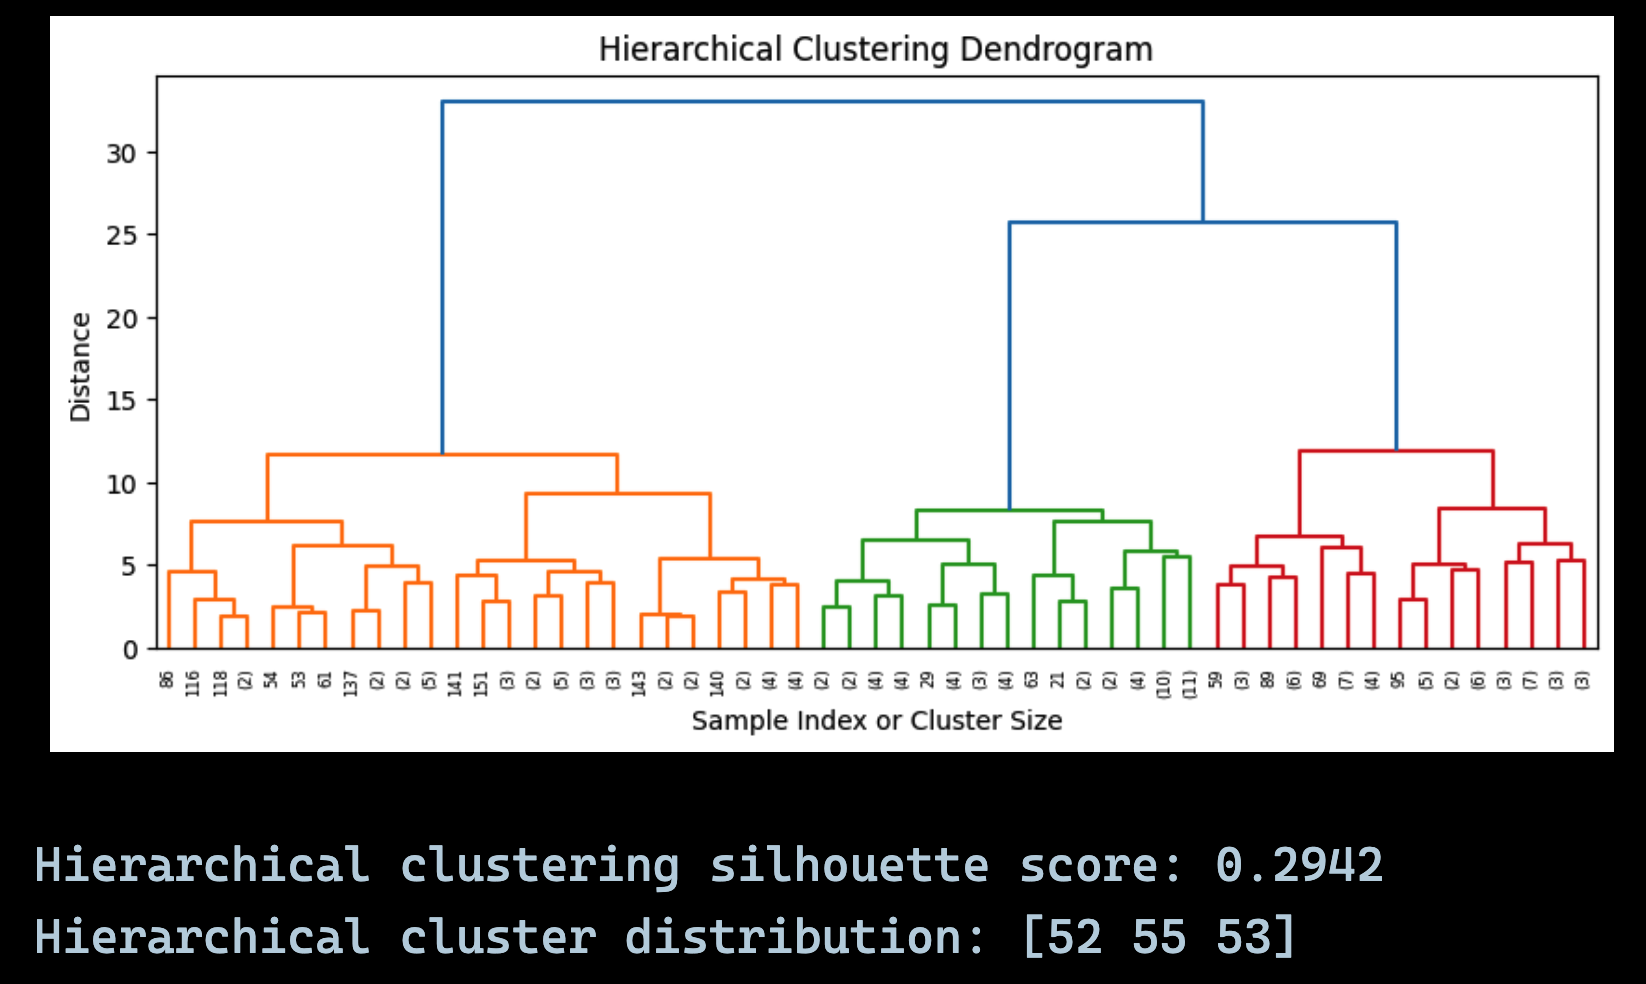
\includegraphics[width=0.95\textwidth]{Figures/dendrogram.png}
    \caption{Hierarchical Clustering Dendrogram and Results}
\end{figure}

\subsubsection{Comparison of Clustering Methods}

\subsubsection{Implementation Approach}
I compared k-means and hierarchical clustering results to understand their differences using side-by-side visualization.

\subsubsection{Implementation Code}
\begin{lstlisting}[language=Python, caption=Clustering Methods Comparison]
# Comparing clustering methods
fig, (ax1, ax2) = plt.subplots(1, 2, figsize=(15, 6))

# K-means visualization
for i in range(3):
    cluster_points = X_pca[cluster_labels == i]
    ax1.scatter(cluster_points[:, 0], cluster_points[:, 1], 
                c=colors[i], label=f'Cluster {i}', alpha=0.7)
ax1.set_title('K-Means Clustering')
ax1.set_xlabel(f'PC1 ({pca.explained_variance_ratio_[0]:.2f} variance)')
ax1.set_ylabel(f'PC2 ({pca.explained_variance_ratio_[1]:.2f} variance)')
ax1.legend()
ax1.grid(True, alpha=0.3)

# Hierarchical clustering visualization
for i in range(3):
    cluster_points = X_pca[hierarchical_labels == i]
    ax2.scatter(cluster_points[:, 0], cluster_points[:, 1], 
                c=colors[i], label=f'Cluster {i}', alpha=0.7)
ax2.set_title('Hierarchical Clustering')
ax2.set_xlabel(f'PC1 ({pca.explained_variance_ratio_[0]:.2f} variance)')
ax2.set_ylabel(f'PC2 ({pca.explained_variance_ratio_[1]:.2f} variance)')
ax2.legend()
ax2.grid(True, alpha=0.3)

plt.tight_layout()
plt.show()
\end{lstlisting}

\subsubsection{Terminal Output}
\begin{figure}[h!]
\centering
    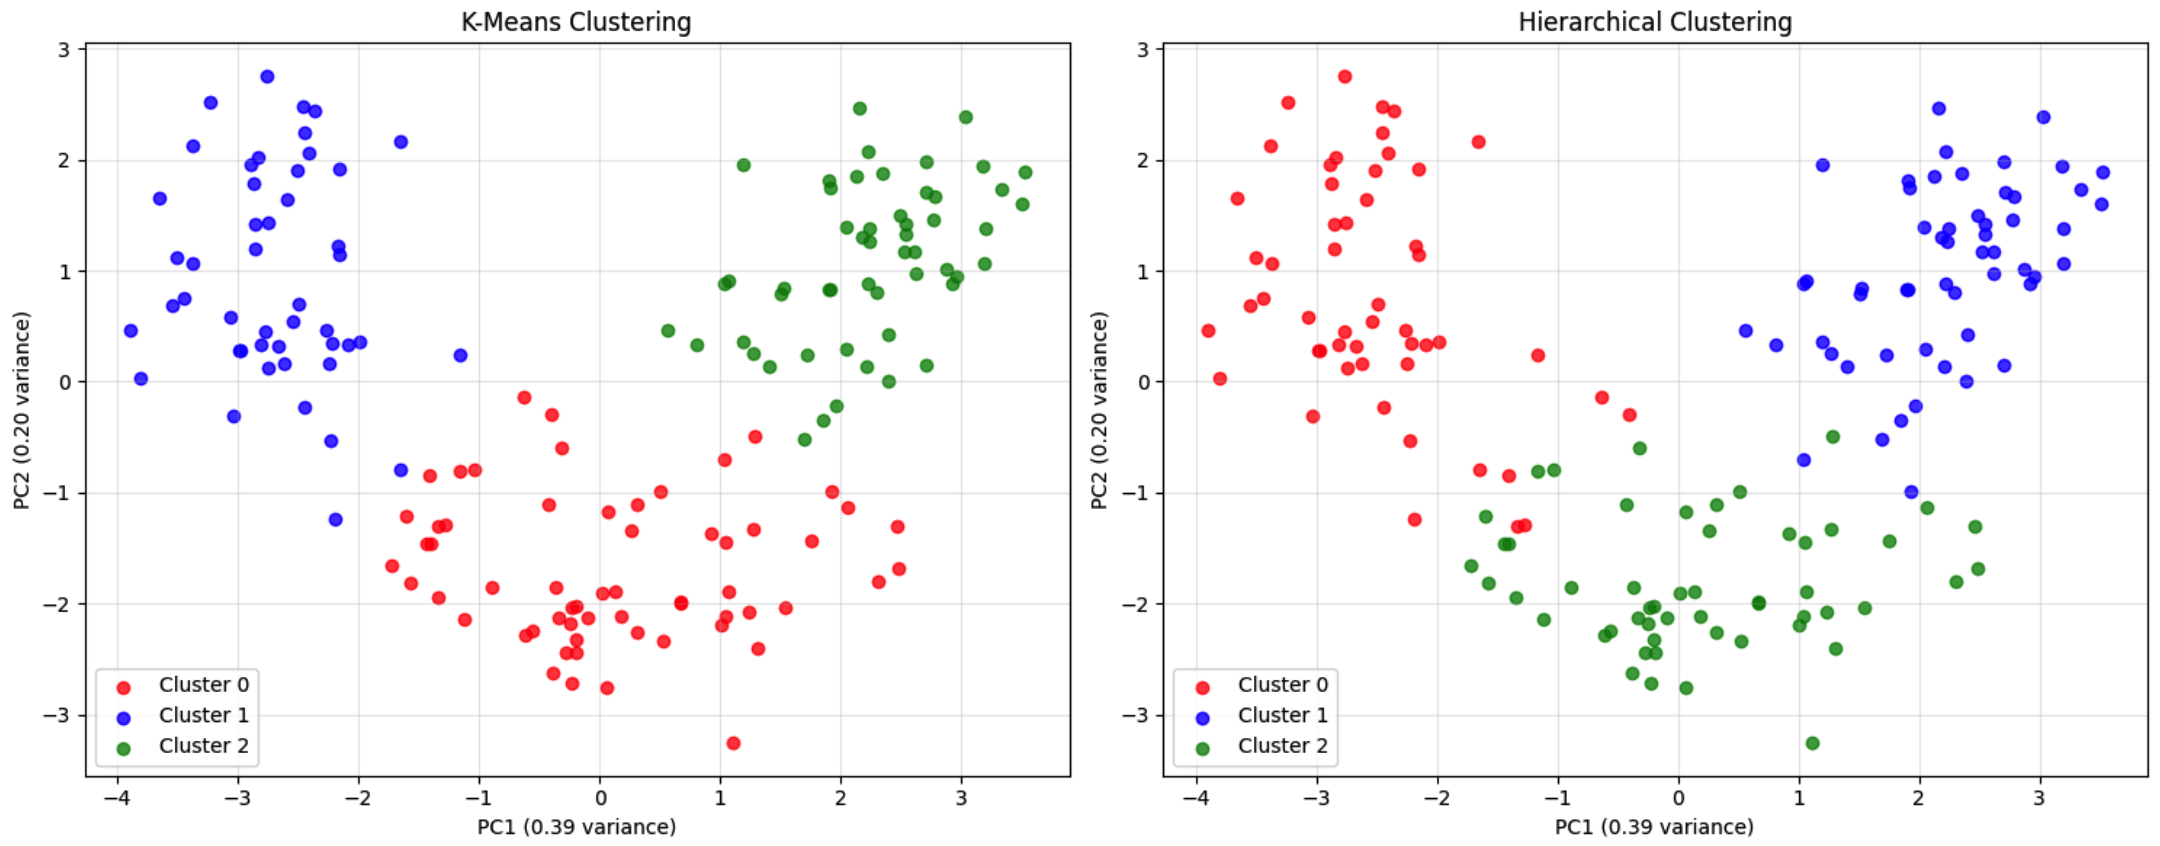
\includegraphics[width=0.95\textwidth]{Figures/clustering_comparison.png}
    \caption{Side-by-Side Comparison of Clustering Methods}
\end{figure}

% ===================== DISCUSSION AND CONCLUSION =====================
\section{Discussion and Conclusion}

This comprehensive laboratory work successfully demonstrated the practical application of both supervised and unsupervised learning techniques through systematic implementation and evaluation of machine learning algorithms on carefully selected datasets. The supervised learning component utilized the renowned Iris dataset to explore classification methodologies, while the unsupervised learning aspect employed the Wine dataset to investigate clustering approaches.

In the classification analysis, both Decision Trees and Na\"{i}ve Bayes algorithms exhibited exceptional performance on the Iris dataset, validating their effectiveness for multi-class classification problems. The Decision Tree implementation, configured with specific parameters including maximum depth of 5, minimum samples split of 10, and minimum samples leaf of 5, achieved robust performance while maintaining excellent interpretability of the decision-making process. The Na\"{i}ve Bayes classifier demonstrated superior accuracy with efficient computational performance, leveraging probabilistic inference to achieve reliable predictions. The application of K-Fold cross-validation with five folds provided comprehensive performance assessment, confirming model stability across different data partitions and validating the generalization capability of both algorithms.

The clustering analysis revealed the effectiveness of unsupervised learning techniques in discovering natural patterns within the Wine dataset. Through careful data preprocessing, including feature standardization and outlier removal using Isolation Forest, the clustering algorithms achieved improved performance and more meaningful results. K-means clustering attained a silhouette score of 0.3004, while hierarchical clustering with Ward linkage achieved 0.2942, both indicating well-separated cluster structures. The implementation of Principal Component Analysis for visualization effectively demonstrated cluster separation in reduced dimensional space, confirming the validity of the identified groupings.

Algorithm selection emerged as a critical factor determining project success, with each method offering distinct advantages suited to specific analytical requirements. Decision Trees provided intuitive decision rules and transparent classification logic, making them ideal for scenarios requiring interpretability. Na\"{i}ve Bayes offered computational efficiency and probabilistic outputs suitable for applications requiring prediction confidence measures. K-means clustering excelled in identifying compact, spherical clusters with balanced distributions, while hierarchical clustering provided valuable structural insights through dendrogram visualization, revealing the hierarchical relationships among data points.

The evaluation methodologies employed throughout this work demonstrated their essential role in comprehensive algorithm assessment. K-Fold cross-validation proved indispensable for reliable performance estimation in supervised learning, while silhouette analysis effectively determined optimal cluster configurations in unsupervised scenarios. The combination of multiple evaluation metrics, including accuracy, precision, recall, and silhouette scores, provided thorough understanding of algorithm behavior and performance characteristics.

This laboratory experience reinforced fundamental principles of successful machine learning implementation, emphasizing the importance of careful algorithm selection based on problem requirements, appropriate data preprocessing techniques, and comprehensive evaluation strategies. The practical skills developed through implementing both supervised classification and unsupervised clustering methodologies establish a solid foundation for addressing diverse machine learning challenges across various application domains.

\end{document}